% Overleaf settings:
% compiler: XeLaTeX

\documentclass[type=bachelor,fontset=custom,pifootnote]{thuthesis}
% 选项:
%   type=[bachelor|master|doctor|postdoctor], % 必选
%   fontset=[fandol|custom],                  % 字体选择
%   secret,                                   % 可选
%   pifootnote,                               % 可选(建议打开)
%   openany|openright,                        % 可选,基本不用
%   arial,                                    % 可选,基本不用
%   arialtoc,                                 % 可选,基本不用
%   arialtitle                                % 可选,基本不用

% **生僻字乱码的解决方法**
% 先解释一下原因: 自带的 fandol 字体不包含生僻字,常用的中易字体因为版权
% 原因不能在 overleaf 发布。
% 解决方法: 找一台 windows 电脑,从 C:\Windows\Fonts 里把
%   simsun.ttc simhei.ttf simkai.ttf simhei.ttf
% 复制出来,上传到 fonts 文件夹,再设置 typeset=custom 即可。


% 所有其它可能用到的包都统一放到这里了,可以根据自己的实际添加或者删除。
\usepackage{thuthesis}

% 定义所有的图片文件在 figures 子目录下
\graphicspath{{figures/}}

% 可以在这里修改配置文件中的定义。导言区可以使用中文。
% \def\myname{文豪}

\usepackage{xeCJKfntef}

\usepackage{amsmath,amsfonts,mathrsfs}
% \usepackage{txfonts}
% \usepackage{mathalfa}

\usepackage{tikz-cd}
\usepackage{tikz}
\usetikzlibrary{shapes,arrows,external,decorations.pathmorphing,backgrounds,positioning,fit,petri,calc,hobby}

% \usetikzlibrary{external}
% \tikzexternalize[prefix=tikz/]
\usepackage{svg}

\usepackage[all]{xy}
\usepackage{xcolor}
\usepackage{cases}
\usepackage{dashbox}

\usepackage{pst-func}

% \usepackage{MnSymbol}

\DeclareMathAlphabet{\mathpzc}{OT1}{pzc}{m}{it}

\newcommand{\qcohsheaf}{^{\mbox{$\sim$}}}
\DeclareMathOperator{\support}{Supp}
\DeclareMathOperator{\coker}{coker}
\DeclareMathOperator{\realpart}{\mathfrak{Re}}
\DeclareMathOperator{\imaginarypart}{\mathfrak{Im}}
\DeclareMathOperator{\gaga}{an}
\DeclareMathOperator{\aut}{Aut}
\DeclareMathOperator{\gl}{GL}
\DeclareMathOperator{\codim}{codim}
\DeclareMathOperator{\gal}{Gal}
\DeclareMathOperator{\diag}{diag}
\newcommand{\resp}{\textit{resp}.\xspace}
\newcommand{\intersect}{\cdot\ldots\cdot}
\DeclareMathOperator{\ann}{Ann}
\DeclareMathOperator{\res}{Res}
\DeclareMathOperator{\proj}{Proj}
\DeclareMathOperator{\PROJ}{\mathbf{Proj}}
\DeclareMathOperator{\car}{car}
\DeclareMathOperator{\Bs}{Bs}
\DeclareMathOperator{\Lb}{B}
\DeclareMathOperator{\des}{des}
\DeclareMathOperator{\sudeg}{\mathrm{su}\widehat{\deg}_{\mathrm{n}}}
\DeclareMathOperator{\udeg}{\mathrm{u}\widehat{\deg}_{\mathrm{n}}}
\DeclareMathOperator{\ndeg}{\widehat{\deg}_{\mathrm{n}}}
\DeclareMathOperator{\Hom}{Hom}
\DeclareMathOperator{\sheafhom}{\mathcal{H}om}
\DeclareMathOperator{\identity}{Id}
\DeclareMathOperator{\Image}{Im}
\DeclareMathOperator{\Pic}{Pic}
\DeclareMathOperator{\pr}{pr}
\DeclareMathOperator{\rg}{rg}
\DeclareMathOperator{\reg}{\mathrm{reg}}
\DeclareMathOperator{\sgn}{sgn}
\DeclareMathOperator{\sing}{\mathrm{sing}}
\DeclareMathOperator{\spec}{Spec}
\DeclareMathOperator{\SPEC}{\mathbf{Spec}}
\DeclareMathOperator{\tr}{Tr}
\DeclareMathOperator{\ord}{ord}
\newcommand{\wmu}{\widehat{\mu}}
\newcommand{\uomega}{\overline{\omega}}
\newcommand{\adeg}{\widehat{\deg}}
\DeclareMathOperator{\sym}{Sym}
\newcommand{\ndot}{\raisebox{.4ex}{.}}

\newcolumntype{P}[1]{>{\centering\arraybackslash}p{#1}}

\allowdisplaybreaks


\begin{document}

%%% 封面部分
\frontmatter
\thusetup{
  %******************************
  % 注意:
  %   1. 配置里面不要出现空行
  %   2. 不需要的配置信息可以删除
  %******************************
  %
  %=====
  % 秘级
  %=====
%   secretlevel={公开},
%   secretyear={0},
  %
  %=========
  % 中文信息
  %=========
  ctitle={自守表示,Langlands 纲领},
  cdegree={理学学士},
  cdepartment={数学科学系},
  cmajor={数理基础科学专业},
  cauthor={文豪},
  csupervisor={印林生\hspace{1em}教授},
  cassosupervisor={}, % 副指导老师
  ccosupervisor={}, % 联合指导老师
  % 日期自动使用当前时间,若需指定按如下方式修改:
   cdate={2010年6月},
  %
  % 博士后专有部分
%   cfirstdiscipline={计算机科学与技术},
%   cseconddiscipline={系统结构},
%   postdoctordate={2009年7月——2011年7月},
%   id={编号}, % 可以留空: id={},
%   udc={UDC}, % 可以留空
%   catalognumber={分类号}, % 可以留空
  %
  %=========
  % 英文信息
  %=========
  etitle={Automorphic Representations, Langlands Program},
  % 这块比较复杂,需要分情况讨论:
  % 1. 学术型硕士
  %    edegree:必须为Master of Arts或Master of Science(注意大小写)
  %             “哲学、文学、历史学、法学、教育学、艺术学门类,公共管理学科
  %              填写Master of Arts,其它填写Master of Science”
  %    emajor:“获得一级学科授权的学科填写一级学科名称,其它填写二级学科名称”
  % 2. 专业型硕士
  %    edegree:“填写专业学位英文名称全称”
  %    emajor:“工程硕士填写工程领域,其它专业学位不填写此项”
  % 3. 学术型博士
  %    edegree:Doctor of Philosophy(注意大小写)
  %    emajor:“获得一级学科授权的学科填写一级学科名称,其它填写二级学科名称”
  % 4. 专业型博士
  %    edegree:“填写专业学位英文名称全称”
  %    emajor:不填写此项
%   edegree={Doctor of Engineering},
%   emajor={Computer Science and Technology},
%   eauthor={Xue Ruini},
%   esupervisor={Professor Zheng Weimin},
%   eassosupervisor={Chen Wenguang},
  % 日期自动生成,若需指定按如下方式修改:
  % edate={December, 2005}
  %
  % 关键词用“英文逗号”分割
  ckeywords={Langlands 纲领, 自守表示, $L$-群, $L$-函数},
  ekeywords={Langlands Program, Automorphic Representations, $L$-group, $L$-functions}
}

% 定义中英文摘要和关键字
\begin{cabstract}
  本文主要介绍了$GL(n)$上的自守表示理论,以及对Langlands纲领进行了一个初步的综述。参照有关的文献,给出了一些基本的结果和主要的猜想。
\end{cabstract}

% 如果习惯关键字跟在摘要文字后面,可以用直接命令来设置,如下:
% \ckeywords{\TeX, \LaTeX, CJK, 模板, 论文}

\begin{eabstract}
   This article mainly introduces the automorphic representation theory for $GL(n)$, and gives an elementary survey of the Langlands Program. Through consulting relevant references, this article presents some fundamental results and conjectures.
\end{eabstract}

% \ekeywords{\TeX, \LaTeX, CJK, template, thesis}

% 如果使用授权说明扫描页,将可选参数中指定为扫描得到的 PDF 文件名,例如:
% \makecover[scan-auth.pdf]
\makecover

%% 目录
\tableofcontents

%% 符号对照表
% \begin{denotation}[3cm]
\item[HPC] 高性能计算 (High Performance Computing)
\end{denotation}



%%% 正文部分
\mainmatter
\chapter{自守表示}
\label{chap:aut_rep}

本章主要介绍的是$GL(n)$的自守表示,因为``自守表示及其$L$-函数是Langlands纲领的核心''\cite{gelbart1984elementary}。本章最终的目的是给出守表示(automorphic representation)以及自守尖点表示(automorphic cuspidal representation)的定义,以及两个大定理Tensor product theorem和Multiplicity one theorem。

\section{一些基本概念}
\label{sec:aut_rep_intro}

我们先来介绍一些基本概念。

设$k$为固定的代数闭域。定义$k$上的$n$维仿射空间\cite{alg_geo}
$$
\mathbb{A}_k^n = \left\{ (a_1,\cdots,a_n) \  \middle| \  a_i\in k, 1 \leqslant i \leqslant n \right\},
$$
赋予$\mathbb{A}_k^n$ Zariski拓扑:取所有予$\mathbb{A}_k^n$所有代数集合的补为予$\mathbb{A}_k^n$的开集。这里,予$\mathbb{A}_k^n$的代数集合被定义为某$n$个变量的$k$系数多项式集合的公共零点集。

\begin{definition}
$\mathbb{A}_k^n$的一个不可约闭子集$X$就称为仿射代数簇。
\end{definition}
这里不可约指的是不能分解成两个真闭子集的并。设$R$为包含$k$的一个环,我们记$X(R)$为坐标取值在$R$中的$X$的点。即设$X = Z(T)$,为多项式集$T$的零点集,那么
$$
X(R) = \left\{ (a_1,\cdots,a_n) \in R^n \  \middle| \ \forall f\in T, f(a_i\in k, 1 \leqslant i \leqslant n) = 0 \right\}.
$$

接下来,我们给出域k上仿射代数群的定义。
\begin{definition}
设$G$为$k$上的一个仿射代数簇,被赋予了一个特殊点$1 \in G(k)$,群的乘法$G \times G \rightarrow G$由多项式给出,使得对任意的包含$k$的环$R$,$G(R)$在这个乘法下成为一个群。那么我们称$G$为域$k$上的一个仿射代数群。
\end{definition}

以下设$F$为一个整体域,即数域或函数域。记$\mathfrak{o}_v$为$F$在$v$处完备化$F_{v}$的整数环。定义$F$的阿代尔环$\mathbb{A}_F$和伊代尔群$\mathbb{A}_F^\times$如下:
\begin{align*}
\mathbb{A}_F & = \left\{ (a_v) \in \prod\limits_v F_v \ \middle|\ \text{对$F$的几乎所有的有限素点$v$有} a_v\in \mathfrak{o}_v \right\}, \\[1em]
\mathbb{A}_F^\times & = \left\{ (a_v) \in \prod\limits_v F_v \ \middle|\ \text{对$F$的几乎所有的有限素点$v$有} a_v\in \mathfrak{o}_v^\times \right\}.
\end{align*}

我们给出表示的相关概念。

\begin{definition}
设$G$为任一群,$V$为某个域$k$上的线性空间。如果存在群同态$\rho: G \rightarrow \operatorname{GL}(V)$,其中$\operatorname{GL}(V)$为一般线性群,那么我们称$(\rho, V)$,简记成$V$或者$\rho$。
\end{definition}
一个等价的定义是$G$在$V$上有一个线性作用,则称$V$为$G$的一个表示。另一个等价的定义是$V$是具有$kG$-模结构,则称$V$为$G$的一个表示。

若$U$是$V$的一个子空间, 且在$G$的作用下为不变子空间, 那么称$(\rho|_U,U)$为$(\rho, V)$的一个子表示。考虑商空间$V/U$,对$g \in G, x + U \in V/U$,定义$g(x + U) = g(x) + U$,那么我们得到$G$在$V/U$上的一个作用,称为$(\rho, V)$的一个商表示,记为$(V/U, \rho_{V/U})$。群$G$的非零表示$(\rho, V)$称为是不可约的,如果他没有非平凡的子表示。

设$(\rho_1, V_1)$和$(\rho_2, V_2)$是群$G$的两个表示,我们称他们是同构的,如果存在单满的$k$-线性映射$f: V_1 \rightarrow V_2$,使得对任一$g \in G$有下面的交换图
\begin{center}
\begin{tikzcd}
V_1 \arrow[r, "f"] \arrow[d, "\rho_1(g)"'] & V_2 \arrow[d, "\rho_2(g)"] \\
V_1 \arrow[r, "f"] & V_2
\end{tikzcd}
\end{center}

关于表示的进一步知识,可以参考\inlinecite{gp_rep}。

现在再来介绍限制直积\cite{nt1}和限制张量积\cite{bump1998automorphic}的概念。

\begin{definition}
设$(G_\lambda)_{\lambda\in\Lambda}$为一族局部紧群,$S$为$\Lambda$的有限子集合,对于每个$\lambda \in \Lambda \setminus S$给定$G_\lambda$的一个紧开子群$U_\lambda$。称直积群$\displaystyle \prod\limits_{\lambda\in\Lambda} G_\lambda$的子群
$$
\left\{ (x_\lambda)_{\lambda\in\Lambda} \in \prod\limits_{\lambda\in\Lambda} G_\lambda  \ \middle|\ \text{对几乎所有$\lambda \in \Lambda \setminus S$有$x_\lambda \in U_\lambda$} \right\}
$$
为$(G_\lambda)_{\lambda\in\Lambda}$关于$(U_\lambda)_{\lambda \in \Lambda \setminus S }$的限制直积。
\end{definition}

我们对限制直积给出如下拓扑。对于包含$S$的$\Lambda$的有限子集$T$,考虑$\prod\limits_{\lambda\in\Lambda} G_\lambda$的子集
$$
G(T) = \prod\limits_{\lambda\in T} G_\lambda \times \prod\limits_{\lambda\in \Lambda \setminus T} U_\lambda.
$$
于是
$$
\prod\limits_{\lambda\in\Lambda} G_\lambda = \bigcup\limits_T G(T).
$$
在每个$G(T)$中引入直积拓扑,对于$\prod\limits_{\lambda\in\Lambda} G_\lambda$的子集$V$,如果对所有$T$,$V \cap
G(T)$为$G(T)$中的开集,则定义$V$为开集。

以下简记$\mathbb{A}_F$为$A$。易知$A$是$F_v$关于$\mathfrak{o}_v$的限制直积。在限制直积拓扑下,$A$是局部紧群。记$A_f$为有限阿代尔组成的环,即
$$
A_f = \left\{ (a_\lambda)_{\lambda\in\Lambda} \in A \ \middle|\ a_v = 1, \text{对所有的无限素点}v \right\}.
$$
同样地,$GL(n, A)$以显然的方式视为$GL(n, F_v)$ 关于$GL(n, \mathfrak{o}_v)$的限制直积。

\begin{definition}
设$\Sigma$为一个指标集,$(V_v)_{v\in\Sigma}$为一族线性空间。对几乎所有的$v\in\Sigma$取定一个非零的$x_v^0 \in V_v$。令$\Omega$为$\Sigma$的满足如下条件的有限子集$S$的集合:若$v\not\in S$,那么$x_v^0$有定义。我们通过包含关系给出$\Omega$的序,那么$\Omega$成为一个定向集。对$S, S'\in\Omega$,且$S \subseteq S'$,我们给出同态:
\begin{figure}[H]
\centering
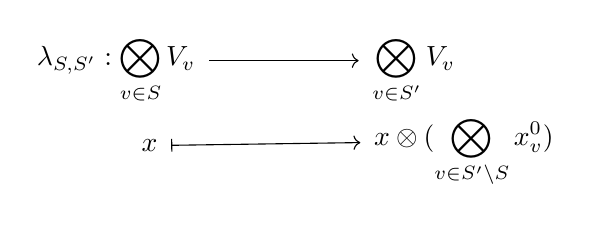
\begin{tikzpicture}
\node[rectangle] (arrow_from) {$\displaystyle \lambda_{S,S'}: \bigotimes\limits_{v\in S} V_v$};
\node[rectangle, right = 2cm of arrow_from] (arrow_to) {$\displaystyle \bigotimes\limits_{v\in S'} V_v$};
\path[->] ([xshift = 0.05cm, yshift=0.12cm]arrow_from.east) edge ([xshift = -0.05cm, yshift=0.12cm]arrow_to.west);

\node[rectangle, below right = 0.21cm and 0.2cm of arrow_from.south] (mapsfrom) {$x$};
\node[rectangle, below left = -0.08cm and -1.9cm of arrow_to.south] (mapsto) {$\displaystyle x\otimes (\bigotimes\limits_{v\in S'\setminus S} x_v^0)$};
\path[|->] ([xshift = 0.05cm]mapsfrom.east) edge ([xshift = -0.05cm, yshift=0.12cm]mapsto.west);
\end{tikzpicture}
\end{figure}
于是我们得到一个正向系统,并称
$$
\bigotimes\limits_v V_v := \varinjlim \bigotimes\limits_{v\in S} V_v
$$
为这一族空间的限制张量积。
\end{definition}

假设我们有一族群$(G_v)_{v\in\Sigma}$,和这族群的子群族$(K_v)_{v\in\Sigma}$。假设对每个$v\in\Sigma$,群$G_v$有一个表示$(V_v,\rho_v)$,并且几乎所有的$v$都存在$\xi_v^0\in V_v$使得$\rho_v(k_v)\xi_v^0 = \xi_v^0$对所有的$k_v \in K_v$成立。令$G$为$G_v$关于$K_v$的限制直积,那么我们可以定义$G$的一个表示$\displaystyle \left( \bigotimes\limits_{v}V_v,  \bigotimes\limits_{v}\rho_v \right)$:
$$
\left(\bigotimes\limits_{v}\rho_v\right) \left( (g_v)_v \right) \left(\bigotimes\limits_{v}x_v\right) = \bigotimes\limits_{v} \rho_v(g_v)x_v.
$$

设$\omega$为$F$的一个Hecke特征,即伊代尔类群的一个特征$\omega: A^\times / F^\times \rightarrow \mathbb{C}_1$。记
$$L^2\left( \operatorname{GL}(n,F)\backslash \operatorname{GL}(n,A), \omega \right)$$
为$\operatorname{GL}(n, A)$上关于其Haar测度\cite{ramakrishnan2005fourier}可测的并且满足如下条件的函数$\phi$组成的线性空间:
\begin{gather}
\label{eq:lin_sp1}
\phi \left( \begin{pmatrix} z & & \\ & \ddots & \\ & & z \end{pmatrix} g \right) = \omega(z)\phi(g), \quad z\in A^\times, \\[1em]
\label{eq:lin_sp2}
\phi(\gamma g) = \phi(g), \quad \gamma \in \operatorname{GL}(n,F), \\[1em]
\int\limits_{Z(A)\operatorname{GL}(n,F)\backslash \operatorname{GL}(n,A)} \lvert \phi(g) \rvert^2 dg < \infty \notag
\end{gather}
这里,$Z(A)$指的是$\operatorname{GL}(n, A)$的中心。$L^2\left( \operatorname{GL}(n,F)\backslash \operatorname{GL}(n,A), \omega \right)$是一个希尔伯特空间。进一步还满足尖点性:对所有的$1 \leqslant r,s \leqslant n-1$,且$r+s=n$,几乎处处成立
\begin{equation}
\label{eq:cusp_cond}
\int\limits_{\operatorname{Mat}_{r\times s}(F) \backslash \operatorname{Mat}_{r\times s}(A)} \phi \left( \begin{pmatrix} I_r & X \\ & I_s \end{pmatrix} g \right) dX = 0
\end{equation}
的$\phi$组成$L^2\left( \operatorname{GL}(n,F)\backslash \operatorname{GL}(n,A), \omega \right)$的一个闭子空间,我们记为
$$L^2_0\left( \operatorname{GL}(n,F)\backslash \operatorname{GL}(n,A), \omega \right).$$
这里$\operatorname{Mat}_{r\times s}$表示$r\times s$矩阵组成的代数群。

我们可以给出$\operatorname{GL}(n,A)$在$L^2\left( \operatorname{GL}(n,F)\backslash \operatorname{GL}(n,A), \omega \right)$上的一个作用$\rho$,即给出表示$\left( L^2\left( \operatorname{GL}(n,F)\backslash \operatorname{GL}(n,A), \omega \right), \rho \right)$。$\rho$的定义如下
$$
(\rho(g)\phi)(x) = \phi(xg), \quad g,x \in \operatorname{GL}(n,A),
$$
即每个$g\in \operatorname{GL}(n,A)$对$L^2\left( \operatorname{GL}(n,F)\backslash \operatorname{GL}(n,A), \omega \right)$的元素的作用是右平移。这个表示称为右正则表示。$L^2_0\left( \operatorname{GL}(n,F)\backslash \operatorname{GL}(n,A), \omega \right)$在这个作用下是一个不变子空间,因此我们得到$\operatorname{GL}(n,A)$的一个子表示。空间$L^2_0\left( \operatorname{GL}(n,F)\backslash \operatorname{GL}(n,A), \omega \right)$具有比较好的性质,我们有如下的定理

\begin{theorem}
$L^2_0\left( \operatorname{GL}(n,F)\backslash \operatorname{GL}(n,A), \omega \right)$可以分解为一些不可约的希尔伯特的不变子
空间的直和。
\end{theorem}

下面我们给出$\operatorname{GL}(n,F)$上自守形式的定义。我们先给定$\operatorname{GL}(n, A)$的一个紧子群$K$:
$$
K = \prod\limits_v K_v, \quad K_v = \begin{cases} O(n), & \text{如果$v$是一个实素点;} \\ U(n), & \text{如果$v$是一个复素点;} \\ \operatorname{GL}(n,\mathfrak{o}_v), & \text{如果$v$是一个有限素点。} \end{cases}
$$
可以证明,$K$是$\operatorname{GL}(n, A)$的一个极大紧子群,并且$\operatorname{GL}(n, A)$的每个极大紧子群都与$K$共轭。

\begin{definition}
我们称$\operatorname{GL}(n, A)$上的函数$\phi$为一个自守形式,如果它满足式\eqref{eq:lin_sp1}和式\eqref{eq:lin_sp2},并且$\phi$还是光滑的,$K$-有限的,$\mathcal{Z}$-有限的,缓慢增长的(of moderate growth)。这里的$\omega$是一个拟特征,被称为自守形式$\phi$的中心拟特征。
\end{definition}
现在来解释后面的几个条件。若$F$是一个函数域,$\phi$是光滑的指的是$\phi$是局部常值的;若$F$为数域,如果对任意的$g\in\operatorname{GL}(n,A)$,存在$g$的一个邻域$N$和$\operatorname{GL}(n,F_\infty)$上的一个光滑函数$\phi_g$,使得对任意$h \in N$,有$\phi(h) = \phi_g(h_\infty)$。这里的
$$F_\infty = \prod\limits_{v\in S_\infty} F_v,$$
$S_\infty$指的是$F$的无穷素点的集合。$\phi$被称为$K$-有限的,如果$K$中元素对$\phi$做右平移张
成的是一个有限维的线性空间。$\mathcal{Z}$是$\operatorname{GL}(n,F_v)$泛包络代数(universal enveloping algebra)的中心\inlinecite{bump1998automorphic}\S 2.2。$\phi$是$\mathcal{Z}$-有限的指的是$\phi$是一个有限维的$\mathcal{Z}$不变空间的元素。$\phi$是缓慢增长的(of moderate growth)指的是对$\operatorname{GL}(n,A)$上的某个高度函数$\lVert\cdot\rVert$,存在常数$C$和$N$,使得对任意的$g\in \operatorname{GL}(n,A)$, $\phi(g) < C\lVert g \rVert^2$。关于后面的这几个条件,具体可参阅\inlinecite{bump1998automorphic} \S 3.3。我们记$\operatorname{GL}(n,A)$上带有中心拟特征$\omega$的自守形式张成的线性空间为
$$\mathcal{A}(\operatorname{GL}(n,F) \backslash \operatorname{GL}(n,A), \omega)$$
进一步,若$\phi$还满足尖点性的条件\eqref{eq:cusp_cond},那么我们称$\phi$为一个尖点形式,并且记尖点形式张成的空间为
$$\mathcal{A}_0(\operatorname{GL}(n,F) \backslash \operatorname{GL}(n,A), \omega)$$

$\mathcal{A}(\operatorname{GL}(n,F) \backslash \operatorname{GL}(n,A), \omega)$在$\operatorname{GL}(n, A_f)$的作用下不变,而且有$(\mathfrak{g}_\infty,  K_\infty)$-模结构。这里的
\begin{gather*}
    \mathfrak{g}_\infty = \prod\limits_{v\in S_\infty} \mathfrak{gl}(n, F), \\[1em]
    K_\infty = \prod\limits_{v\in S_\infty} K_v
\end{gather*}
$\mathfrak{gl}(n, F)$为李代数。在这个意义下$\mathcal{A}(\operatorname{GL}(n,F) \backslash \operatorname{GL}(n,A), \omega)$成为$\operatorname{GL}(n,A)$的一
个``表示''。严格来说$\mathcal{A}(\operatorname{GL}(n,F) \backslash \operatorname{GL}(n,A), \omega)$和$\mathcal{A}_0(\operatorname{GL}(n,F) \backslash \operatorname{GL}(n,A), \omega)$并不是$\operatorname{GL}(n,A)$的表示,而是$\operatorname{GL}(n,A)$的整体Hecke代数$\mathcal{H}_{\operatorname{GL}(n,A)}$的表示,见\inlinecite{bump1998automorphic}的\S 3.4。

下面,我们给出自守表示(automorphic representation) 以及自守尖点表示(automorphic cuspidal representation)的定义。

\begin{definition}[自守表示]
我们称$\operatorname{GL}(n,A)$的一个不可约表示为自守表示,如果他同构于$\mathcal{A}(\operatorname{GL}(n,F) \backslash \operatorname{GL}(n,A), \omega)$的某个子表示的商。
\end{definition}

\begin{definition}[自守尖点表示]
我们称$\operatorname{GL}(n,A)$的一个不可约表示为自守表示,如果他同构于$\mathcal{A}_0(\operatorname{GL}(n,F) \backslash \operatorname{GL}(n,A), \omega)$的某个子表示的商。
\end{definition}

\section{主要的定理}

现在我们给出本章的主要定理。首先我们给出一些引理和定义。

\begin{lemma}
设$(\rho, V)$为$K$的一个有限维不可约表示,那么存在$K_v$的一个有限维表示$(\rho_v, V_v)$,使得对几乎所有的$v$,$(\rho_v, V_v)$是$K_v$的平凡表示,而且存在$\xi_v^0\in V_v$,,使得$(\rho, V)$同构于$(\otimes_{v}\rho_v, \otimes_v V_v)$,其中$\otimes_v V_v$是是关于$(V_v,\xi_v^0)_v$的限制张量积。
\end{lemma}
这个引理说的是$K$的有限维不可约表示总可以写成每个局部的有限维不可约表示的限制张量积。

\begin{proof}
由于
$$K_f := \prod\limits_{v \not \in S_\infty}$$
是完全不连通的,可以证明对满足引理条件的表示$\rho$,$\ker \rho$包含K的一个开子群,因此包含几乎所有的$K_v$。令$S$为包含$S_\infty$的一个有限集合,使得对所有的$v \not \in S$,有$\rho(K_v)=1$,即$\rho$在这些$K_v$上是平凡的。于是
$$K / [ \prod\limits_{v \not\in S} K_v ] \cong \prod\limits_{v \in S} K_v $$
对$V$有作用,并且这个表示也是不可约的。

$\prod\limits_{v \in S} K_v$是一个紧群的有限直积, 而他所有的不可约表示都可以分解成$\otimes_{v\in S}\rho_v$,$\rho_v$是$K_v$的不可约表示。对$v\not\in S$,我们取$(\rho_v, V_v)$为$K_v$的平凡表示。这样,$\rho$就与$\otimes_{v\in S}\rho_v$同构了。引理中的$\xi_v^0$可取为$V_v$任何一个元,$v \not\in S$。
\end{proof}

\begin{definition}
设$(\pi, V)$为$K$的一个表示,设$(\rho, V_\rho)$为$K$的一个有限维不可约表示。令$V(\rho)$为$V$的所有同构于$V_\rho$的子表示的和。我们称$V(\rho)$为表示$(\pi, V)$的$\rho$-同型($\rho$-
isotypic)部分。
\end{definition}

设$V$为一个复线性空间,同时是

\chapter{Langlands猜想}
\label{chap:langlands}

待添加

\chapter{总结}
\label{chap:summary}

待添加



%%% 其它部分
\backmatter

% %% 本科生要这几个索引,研究生不要。选择性留下。
% % 插图索引
% \listoffigures
% % 表格索引
% \listoftables
% % 公式索引
% \listofequations


%% 参考文献
% 注意:至少需要引用一篇参考文献,否则下面两行可能引起编译错误。
% 如果不需要参考文献,请将下面两行删除或注释掉。
\bibliographystyle{thuthesis-numerical}
\bibliography{ref/refs}


%% 致谢
% 如果使用声明扫描页,将可选参数指定为扫描后的 PDF 文件名,例如:
% \begin{ack}[scan-statement.pdf]
\begin{acknowledgement}
  衷心感谢导师印林生教授对本人的精心指导。他的言传身教将使我终生受益。

  感谢 \thuthesis,它的存在让我的论文写作轻松自在了许多,让我的论文格式规整漂亮了
  许多。
\end{acknowledgement}


%% 附录
% \begin{appendix}
% \chapter{外文资料原文}
\label{cha:engorg}


% \end{appendix}

%% 个人简历
% \begin{resume}

  \resumeitem{个人简历}

  xxxx 年 xx 月 xx 日出生于 xx 省 xx 县。

  xxxx 年 9 月考入 xx 大学 xx 系 xx 专业,xxxx 年 7 月本科毕业并获得 xx 学士学位。

  xxxx 年 9 月免试进入 xx 大学 xx 系攻读 xx 学位至今。

%   \researchitem{发表的学术论文} % 发表的和录用的合在一起

%   % 1. 已经刊载的学术论文(本人是第一作者,或者导师为第一作者本人是第二作者)
%   \begin{publications}
%     \item Yang Y, Ren T L, Zhang L T, et al. Miniature microphone with silicon-
%       based ferroelectric thin films. Integrated Ferroelectrics, 2003,
%       52:229-235. (SCI 收录, 检索号:758FZ.)
%     \item 杨轶, 张宁欣, 任天令, 等. 硅基铁电微声学器件中薄膜残余应力的研究. 中国机
%       械工程, 2005, 16(14):1289-1291. (EI 收录, 检索号:0534931 2907.)
%     \item 杨轶, 张宁欣, 任天令, 等. 集成铁电器件中的关键工艺研究. 仪器仪表学报,
%       2003, 24(S4):192-193. (EI 源刊.)
%   \end{publications}

%   % 2. 尚未刊载,但已经接到正式录用函的学术论文(本人为第一作者,或者
%   %    导师为第一作者本人是第二作者)。
%   \begin{publications}[before=\publicationskip,after=\publicationskip]
%     \item Yang Y, Ren T L, Zhu Y P, et al. PMUTs for handwriting recognition. In
%       press. (已被 Integrated Ferroelectrics 录用. SCI 源刊.)
%   \end{publications}

%   % 3. 其他学术论文。可列出除上述两种情况以外的其他学术论文,但必须是
%   %    已经刊载或者收到正式录用函的论文。
%   \begin{publications}
%     \item Wu X M, Yang Y, Cai J, et al. Measurements of ferroelectric MEMS
%       microphones. Integrated Ferroelectrics, 2005, 69:417-429. (SCI 收录, 检索号
%       :896KM)
%     \item 贾泽, 杨轶, 陈兢, 等. 用于压电和电容微麦克风的体硅腐蚀相关研究. 压电与声
%       光, 2006, 28(1):117-119. (EI 收录, 检索号:06129773469)
%     \item 伍晓明, 杨轶, 张宁欣, 等. 基于MEMS技术的集成铁电硅微麦克风. 中国集成电路,
%       2003, 53:59-61.
%   \end{publications}

%   \researchitem{研究成果} % 有就写,没有就删除
%   \begin{achievements}
%     \item 任天令, 杨轶, 朱一平, 等. 硅基铁电微声学传感器畴极化区域控制和电极连接的
%       方法: 中国, CN1602118A. (中国专利公开号)
%     \item Ren T L, Yang Y, Zhu Y P, et al. Piezoelectric micro acoustic sensor
%       based on ferroelectric materials: USA, No.11/215, 102. (美国发明专利申请号)
%   \end{achievements}

\end{resume}

\end{document}
